Table \ref{ch:DAIL:tab:Reward_Simple} reports the quantitative evaluations of the proposed \DAIL{} agent on low-dimensional tasks, in terms of average cumulative rewards.
The numerical results clearly indicate that, for all evaluated tasks, TRPO \cite{RL_TRPO} provided the best performance as its average cumulative rewards were at the highest.
This was actually predictable because TRPO \cite{RL_TRPO} had direct access to states and shaped rewards of the learner domain.
On the other hand, inputs of GAMA-PA \cite{DAIL_Model_DAIL} and \DAIL{} were limited to expert demonstrations only.
As a result, their performances deteriorated compared to TRPO \cite{RL_TRPO}.
However, Table \ref{ch:DAIL:tab:Reward_Simple} also determines that the proposed \DAIL{} outperformed GAMA-PA \cite{DAIL_Model_DAIL} across all three tasks.
Additionally, for the Pendulum-Acrobot task, the proposed agent almost achieved as high performance as TRPO \cite{RL_TRPO}.
In order to understand the observed results more deeply, Figures \ref{ch:DAIL:fig:PendulumAcrobot}, \ref{ch:DAIL:fig:PendulumCartPole} and \ref{ch:DAIL:fig:AcrobotCartPole} visualize the behaviors of learned policies provided by the evaluated agents when performing the Pendulum-Acrobot, Pendulum-CartPole and Acrobot-CartPole tasks, respectively.

\begin{table}[htbp!]
  \centering
  \caption{\added{The performance of the proposed \DAIL{} agent on low-dimensional tasks. These scores represent the cumulative rewards obtained from executing a learned policy in the simulator, averaged over 100 episodes.}}
  \label{ch:DAIL:tab:Reward_Simple}
  % TRPO
% Pendulum:
%       Mean:  -135.73463514842086    Std:  83.24276932922322
% CartPole:
%       Mean:  497.13       Std:  28.55613944496
% Acrobot:
%       Mean:  -63.18       Std:  7.047524388038681

% GAMA
% Acrobot:
%       Mean: -386.31   Std: 49.20
% Pendulum-CartPole:
%       Mean:  144.03   Std:  89.08574016081361
% Acrobot-CartPole:
%       Mean: 1
% Our
% Acrobot:
%       Mean:  -83.31   Std:  32.61248073974134
% Pendulum-CartPole:
%       Mean:  289.74   Std:  171.20727905086278
% Acrobot-CartPole:
%       Mean:  153.86 Std:  81.79371294405652
%

\begin{tabular}{cccc}
  \toprule
  \textbf{Task}     & \textbf{\DAIL{}}    & \textbf{GAMA-PA\cite{DAIL_Model_DAIL}} & \textbf{TRPO} \cite{RL_TRPO} \\
  \midrule
  Pendulum-Acrobot  & -83.31 $\pm$  32.61 & -386.31 $\pm$ 49.20                    & -63.18 $\pm$  7.05           \\
  Pendulum-CartPole & 289.74 $\pm$ 171.21 & 144.03 $\pm$ 89.09                     & 497.13 $\pm$ 28.56           \\
  Acrobot-CartPole  & 153.86 $\pm$  81.79 & 93.05 $\pm$ 88.97                      & 497.13 $\pm$ 28.56           \\
  \bottomrule
\end{tabular}

\end{table}

\begin{landscape}
  \begin{figure}[htbp!]
    \centering
    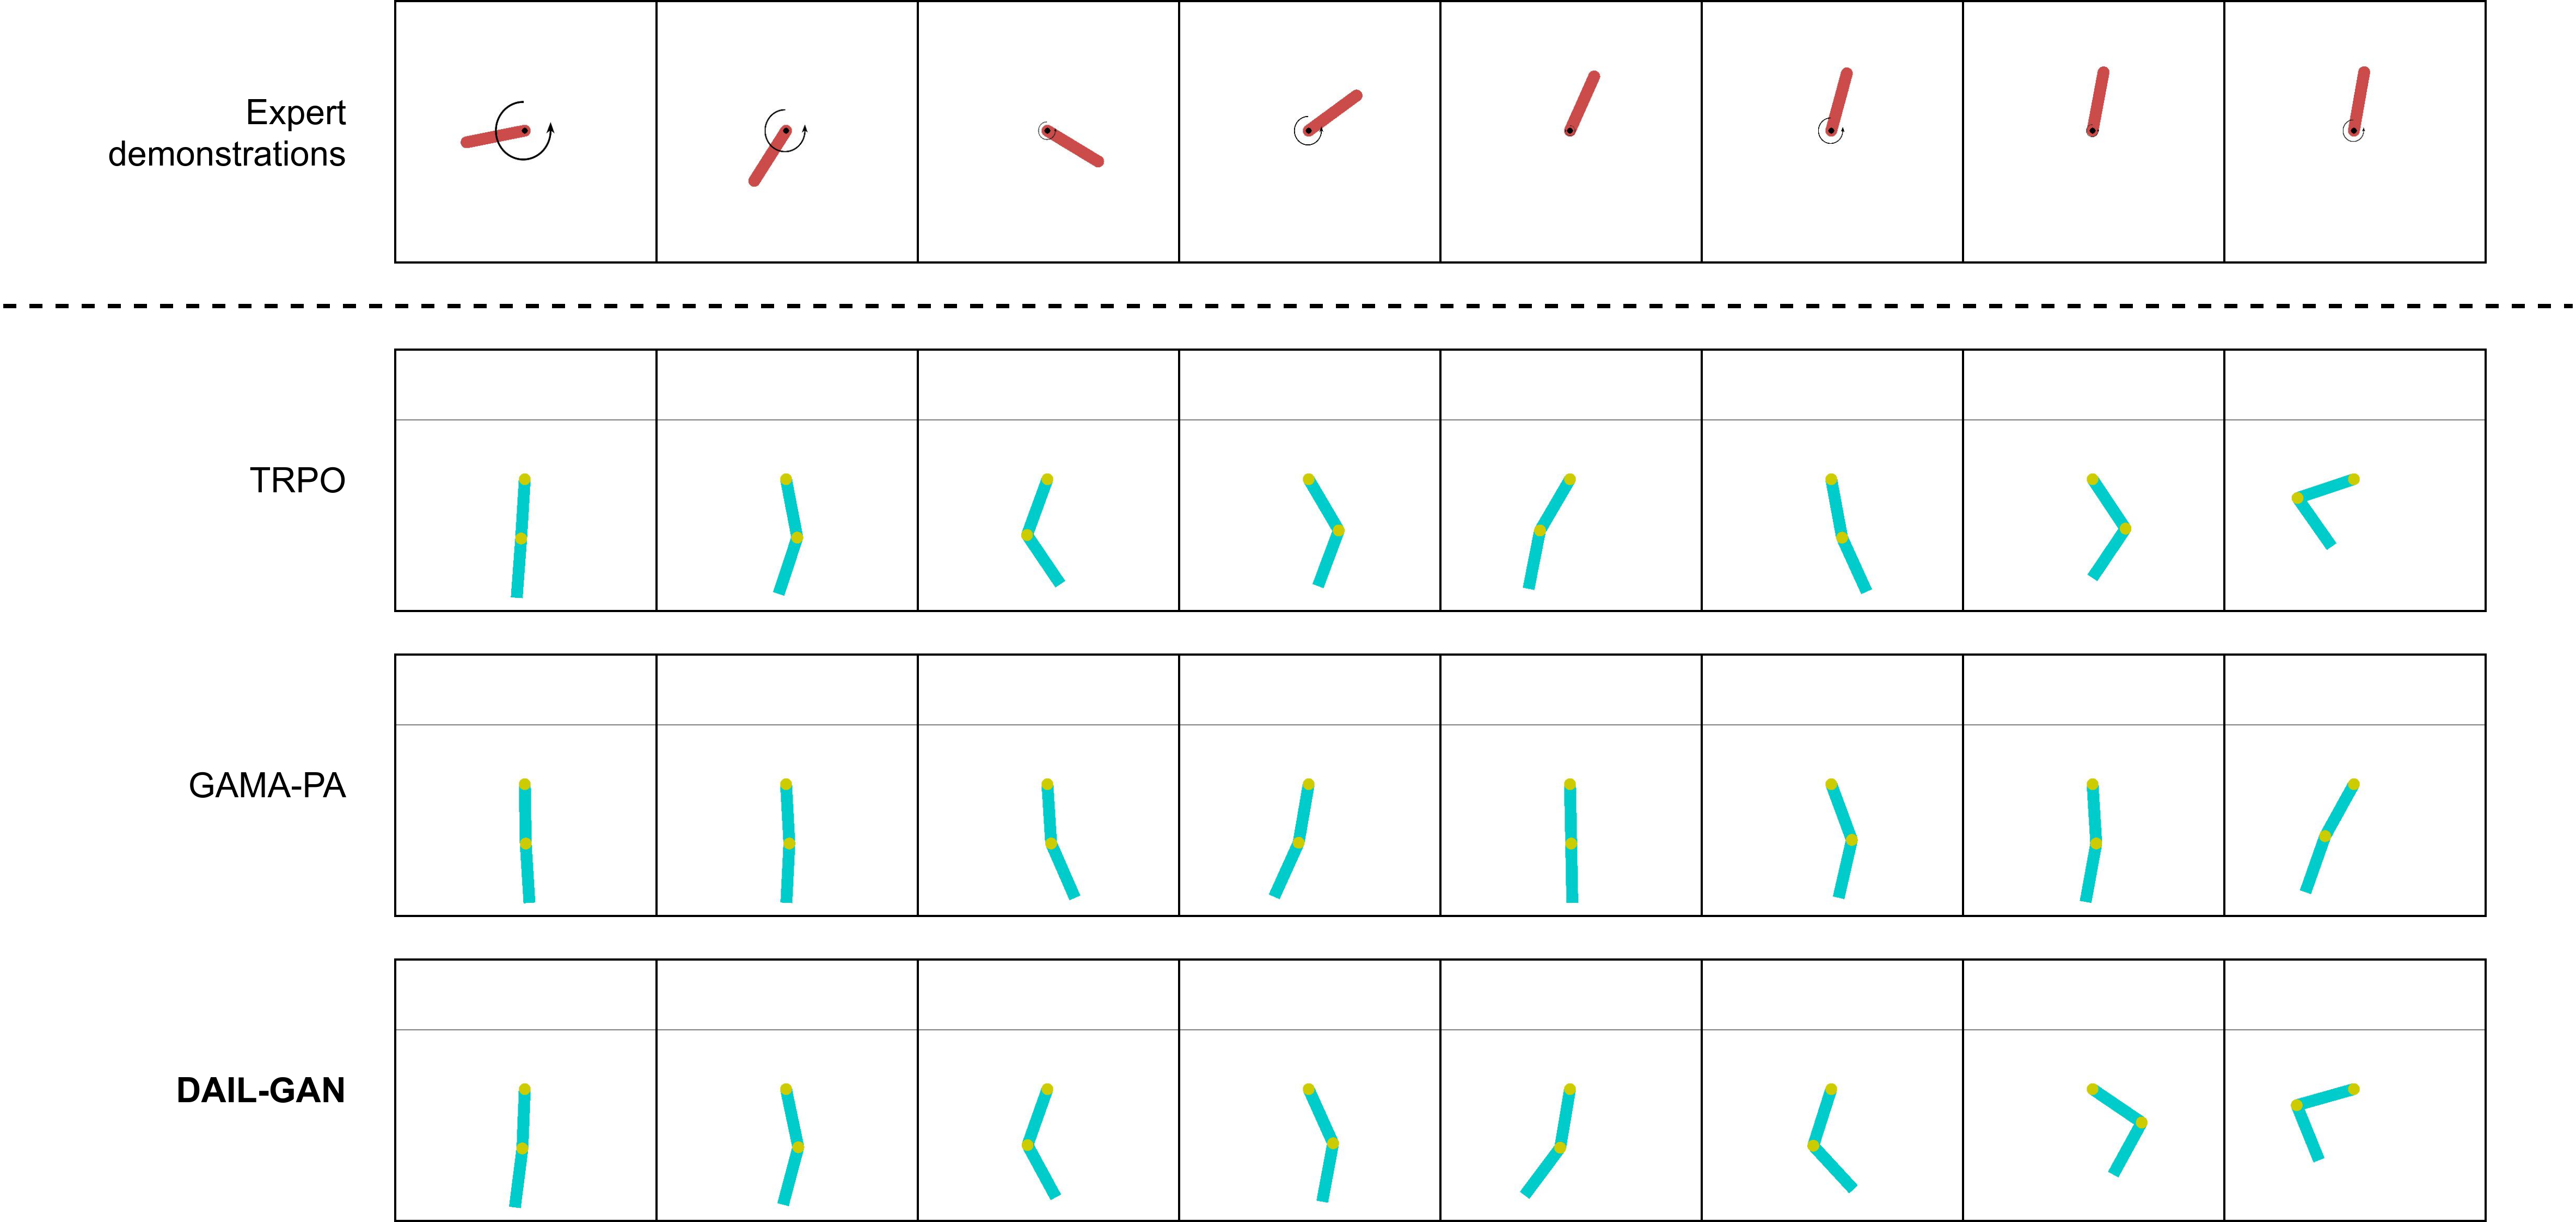
\includegraphics[width=0.7\pdfpageheight]{\FigsDir/Pendulum-Acrobot.png}
    \caption{Pendulum-Acrobot.}
    \label{ch:DAIL:fig:PendulumAcrobot}
  \end{figure}
\end{landscape}


\begin{landscape}
  \begin{figure}[htbp!]
    \centering
    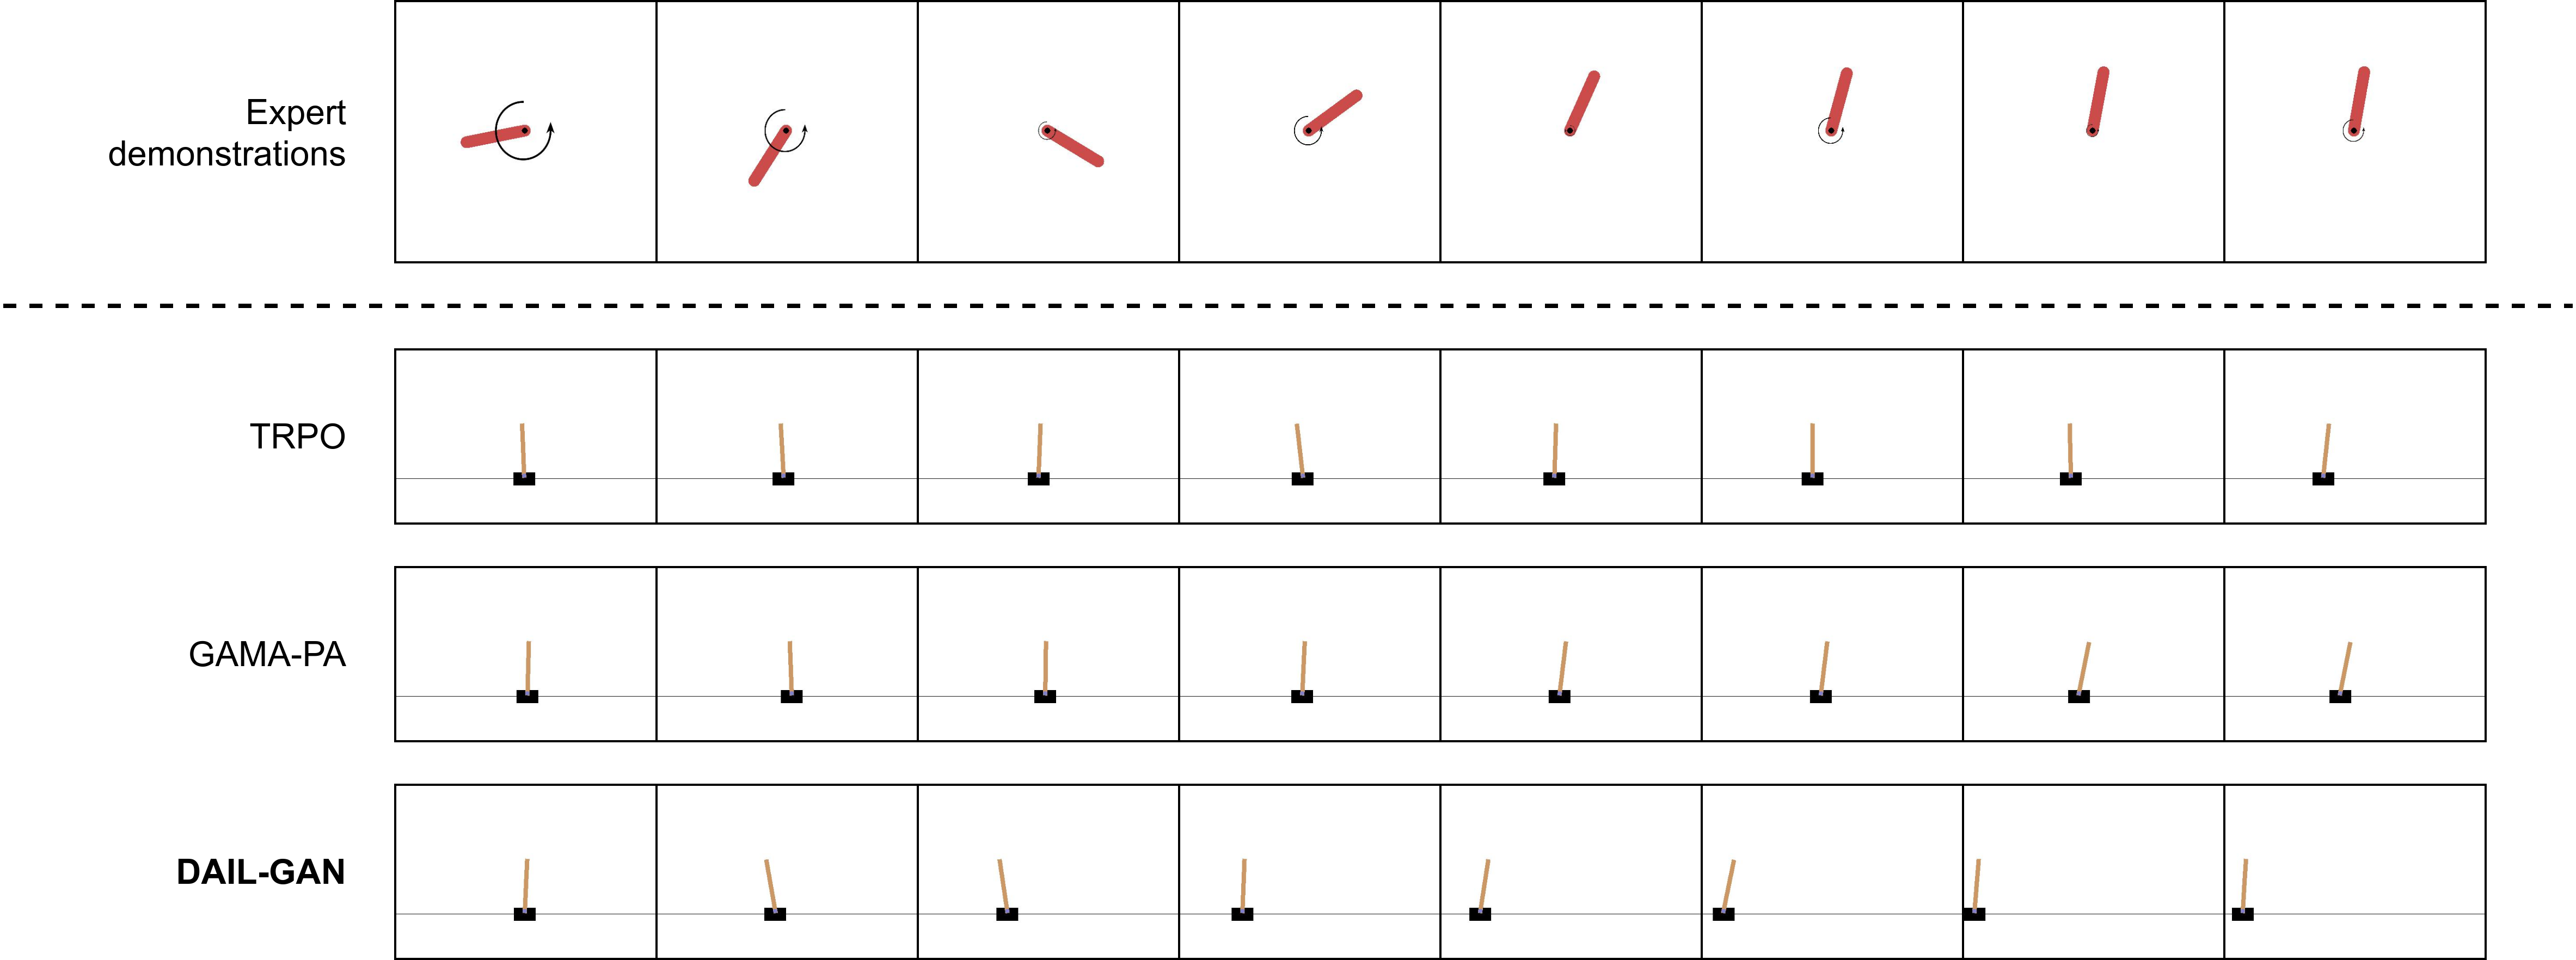
\includegraphics[width=0.7\pdfpageheight]{\FigsDir/Pendulum-CartPole.png}
    \caption{Pendulum-CartPole.}
    \label{ch:DAIL:fig:PendulumCartPole}
  \end{figure}
\end{landscape}

\begin{landscape}
  \begin{figure}[htbp!]
    \centering
    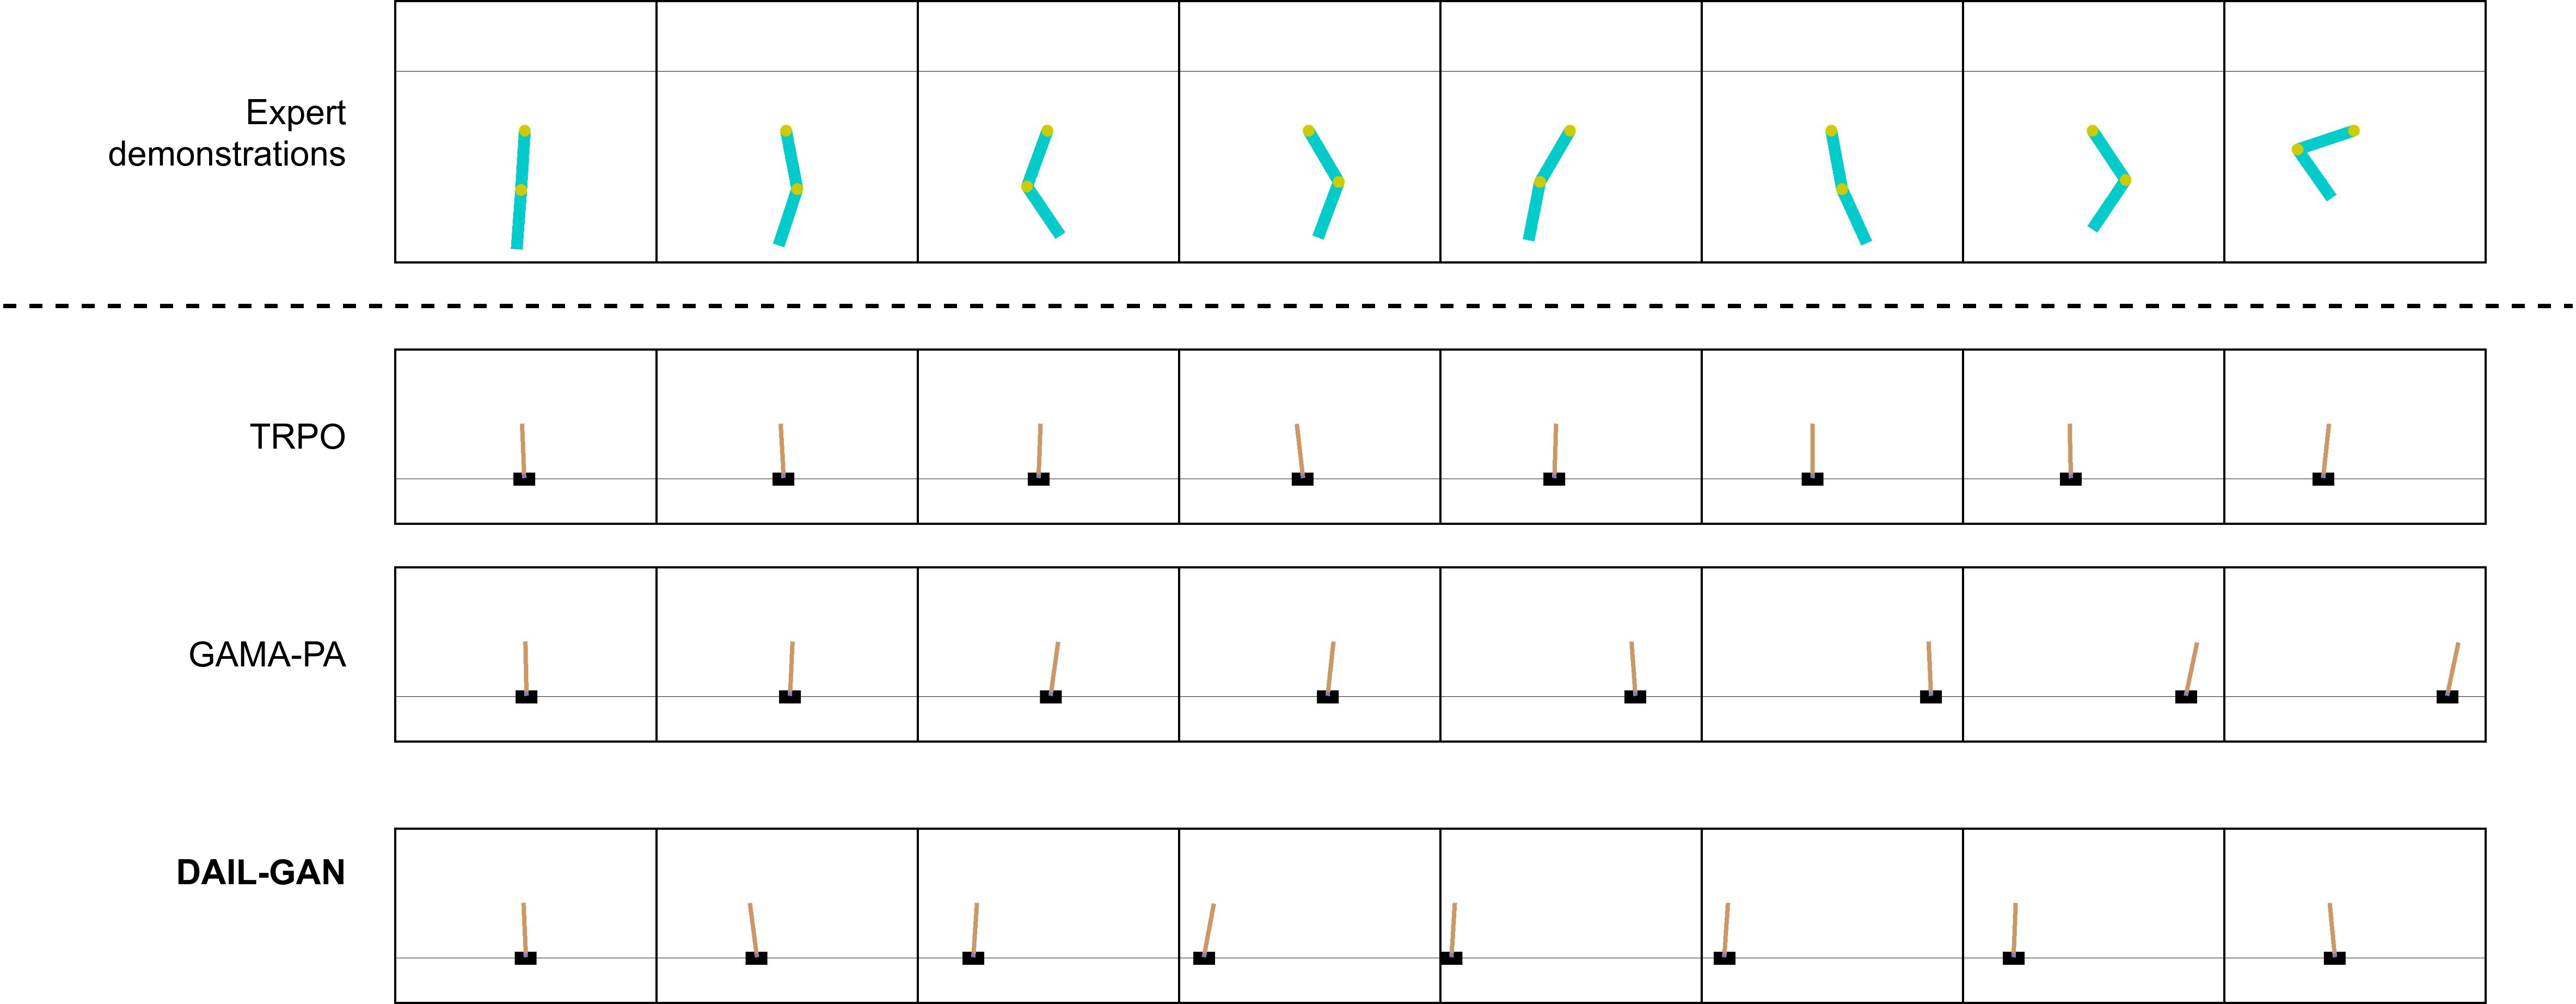
\includegraphics[width=0.7\pdfpageheight]{\FigsDir/Acrobot-CartPole.png}
    \caption{Acrobot-CartPole.}
    \label{ch:DAIL:fig:AcrobotCartPole}
  \end{figure}
\end{landscape}

In the expert demonstration of the Pendulum-Acrobot task in Figure \ref{ch:DAIL:fig:PendulumAcrobot} and the Pendulum-CartPole task in Figure \ref{ch:DAIL:fig:PendulumCartPole}, expert behaviors were to apply a strong force, expressed by a rotation velocity, at first to make the pendulum swing upright.
After that, a few light forces were applied to maintain it vertically.
Observing from Figure \ref{ch:DAIL:fig:PendulumAcrobot}, the policies trained with GAMA-PA \cite{DAIL_Model_DAIL} failed to apply strong enough forces to swing the lower link as high as the proposed DAIL.
Also, Figure \ref{ch:DAIL:fig:PendulumCartPole} expresses that the GAMA-PA \cite{DAIL_Model_DAIL} could not move the cart at an appropriate velocity to keep the pole stay vertical.
It was because the expert demonstration also did not show much movement after successfully swinging the pendulum upright as it only applied light forces.
Meanwhile, the policies learned by the \DAIL{} agent could accomplish the task.
Interestingly, it can be observed that the learned policies are able to produce behaviors that relatively similar to the expert: the cart was first pushed to the left by a strong force, then small forces are applied to prevent the pole from falling over.

For the Acrobot-CartPole task in Figure \ref{ch:DAIL:fig:AcrobotCartPole}, the behaviors of the expert were that the link was swung back and forth to gain enough velocity to reach a higher height.
Similarly, the GAMA-PA's learned policy could move the cart faster compared to the Pendulum-CartPole task.
Yet, it still failed to maintain appropriate velocity to keep the pole standing.
On contrary, the proposed \DAIL{} was able to remain the pole vertical.
It is important to note that the learned policy of \DAIL{} could move the cart in both directions which is also similar to the expert behaviors.

The above observations show that the proposed \DAIL{} agent not only succeeded in imitating the expert behaviors but also adapted the learned policies well to a distinct learner domain.
Meanwhile, although the GAMA-PA \cite{DAIL_Model_DAIL} could learn the state -- action maps from expert to learner domain, its adaptation algorithm was inefficient to help it accomplish the tasks.
